% Preamble
% Compile with XeLateX

\documentclass[11 pt,oneside,a4paper,titlepage]{article}
\usepackage{preamble}
\graphicspath{{PIC/}}
\usepackage{zh_CN-Adobefonts_external}

%%%%%%%%%%%%%%%%%%%%%%%%%%%%%%%%%%%%%%%%%%%%%%%%%%%%%%%%%%%%%%%%%%%%%%%%%%%%%%%%%%%%%%
\begin{document}

\sidebar{sideBarColor!25}
\simpleheader{titleBackColor}{彥翔}{林}{2024 英國伯明翰大學碩士應屆畢業生|多益:955|雅思學術:7|歐盟航空安全總署 Part-147 核准證書}{white}

% Start Minipages
\vspace*{3.49cm}
    \adjustbox{valign=t}{\begin{minipage}{6.7cm}
    \vspace*{0.6cm}
            
        % Picture
        \begin{center}
        \begin{tikzpicture}
            \node[
            circle,
            minimum size=\cvPictureWidth,
            path picture={
            \node at (path picture bounding box.center){
             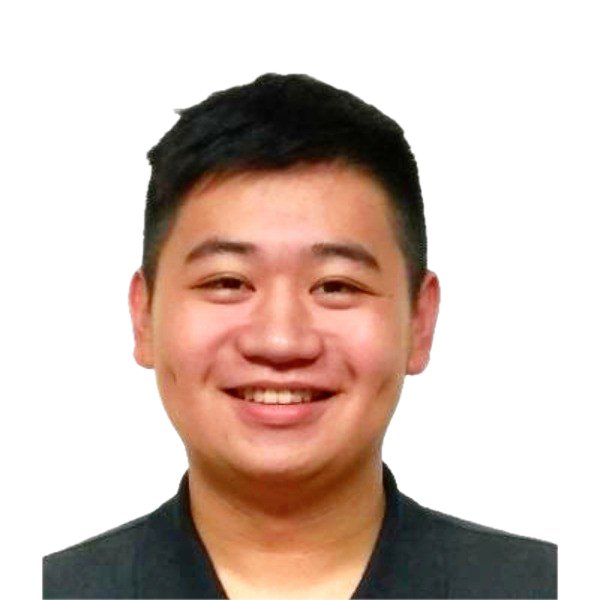
\includegraphics[width=\cvPictureWidth]{Picture.png}
             };
             }]
            {};
        \end{tikzpicture}
        \end{center}
        %%%%%%%%%%%%%%%%%%%%%%%%%%%%%%%%%%%%%%%%%%%%%%%%%%%%
        % Profile section
        \ruleline{\textbf{\color{titleBackColor} 關於我}}
        科技一直深深吸引著我,尤其是精密和先進系統的交集。
        \newline
        作為一名英國伯明翰大學的碩士應屆畢業生,我擁有高度的上進心和適應能力。我的學經歷雖然非比尋常,但卻讓我獨特地擁有了結合精準、嚴謹技術和創新的多樣化技能。從複雜的飛機修護到最前沿的電腦科學,我在硬體和軟體兩方面都建立了穩固的基礎,並且我渴望將這種獨特的融合帶入半導體產業。
        %%%%%%%%%%%%%%%%%%%%%%%%%%%%%%%%%%%%%%%%%%%%%%%%%%%
        \ruleline{\textbf{\color{titleBackColor} 語言能力}}
        \begin{tikzpicture}[every node/.style={inner sep=0pt, outer sep=0pt}]
        \matrix [
        column 1/.style={anchor=center,contactIcon},
        column 2/.style={anchor=west,align=left,contactIcon},
        column sep=5pt,
        row sep=5pt] (contact) {
        \node{\flag{England.png}};
        & \node{英文 - 多益:955,雅思學術:7};\\
        \node{\flag{taiwan.png}};
        & \node{中文 - 母語};\\
        };
        \end{tikzpicture} 
        %%%%%%%%%%%%%%%%%%%%%%%%%%%%%%%%%%%%%%%%%%%%%%%%%%%
        % Contact Section
        \ruleline{\textbf{\color{titleBackColor} 聯絡資料}}
        \begin{tikzpicture}[every node/.style={inner sep=0pt, outer sep=0pt}]
        \matrix [
        column 1/.style={anchor=center,contactIcon},
        column 2/.style={anchor=west,align=left,contactIcon},
        column sep=5pt,
        row sep=5pt] (contact) {
        \node{\circled{\faAddressCard}};
         & \node{生於:1999/07/07,25歲};\\
         & \node{兵役狀態:2024/10/31 入伍;\\\hspace{1.075cm}預計 2025/02/25 退伍};\\
        \node{\circled{\faCar}};
         & \node{普通小型車, 手/自排A 類駕照};\\
        \node{\circled{\faStreetView}};
         & \node{\href{https://www.google.com/maps/place/Zhongli+District,+Taoyuan+City,+Taiwan}{\textcolor{blue}{\underline{中壢區,桃園市,台灣} \footnotesize\faIcon{external-link-alt}}}};\\
        \node{\circled{\faEnvelope}}; 
         & \node{\href{mailto:yxl1751@alumni.bham.ac.uk}{\textcolor{blue}{\underline{yxl1751@alumni.bham.ac.uk} \footnotesize\faIcon{external-link-alt}}}};\\
        \node{\circled{\faIcon{mobile-alt}}}; 
         & \node{\href{tel:+886908890707}{\textcolor{blue}{\underline{(+886) 908 890 707} \footnotesize\faIcon{external-link-alt}}}};\\
        \node{\circled{\faIcon{mobile-alt}}}; 
         & \node{\href{tel:+447593742667}{\textcolor{blue}{\underline{(+44) 7593 742667} \footnotesize\faIcon{external-link-alt}}}};\\
        \node{\circled{\faLinkedin}}; 
         & \node{\href{https://linkedin.com/in/yen-hsiang-lin/}{\textcolor{blue}{\underline{linkedin.com/in/yen-hsiang-lin} \footnotesize\faIcon{external-link-alt}}}};\\
        \node{\circled{\faGithub}};
         & \node{\href{https://github.com/Ethan-YanXiang/}{\textcolor{blue}{\underline{github.com/Ethan-YanXiang} \footnotesize\faIcon{external-link-alt}}}};\\
         };
        \end{tikzpicture}
        %%%%%%%%%%%%%%%%%%%%%%%%%%%%%%%%%%%%%%%%%%%%%%%%%%%%%
        % QR Code
        \ruleline{\textbf{\color{titleBackColor} 領英 QR碼}}
        % \scriptsize
        \begin{center}
            \qrcode[height=2.5cm]{https://linkedin.com/in/yen-hsiang-lin/} \\ %height=2.5cm
            \vspace*{0.6cm}
            掃一下 \space 發現更多 \faLinkedin \\
        \end{center}
        
    \end{minipage}} %
    \hfill 
%%%%%%%%%%%%%%%%%%%%%%%%%%%%%%%%%%%%%%%%%%%%%%%%%%%%%%%%%
%%%%% MAIN SECTION %%%%%%%%%%%%%%%%%%%%
    \adjustbox{valign=t}{\begin{minipage}{13.1cm}
        \vspace*{.7cm}
        % Work Experience
        \noindent
        \section*{\resheading{\textbf{{\faToolbox} 工作經歷}}}

        \MySectionNoPic{2020/09\\ \faAngleDoubleDown \\2021/05}{LTT.png}{CAA \& EASA 許可的飛機修護工程計劃}{德國漢莎航空技術訓練}{新竹,台灣}{學徒}
        {\begin{itemize}[label=\Large\textbullet]
            \item 事先研究並熟悉不同手冊中與指定任務相關的所有章節,視需求依據料號/件號手冊到庫房領取替換件或耗材
            \item 依照標準作業程序,將飛機頂舉並更換機輪和煞車碟盤,執行減震支柱液壓油補充及氮氣充填服務
            \item 根據結構修理手冊的規範進行蒙皮修復,包括判定損傷是否在允許範圍內以及應用補片修復
            \item 與夥伴培養默契,在時間限制下進行維修檢查,並完成測試
            \item 在完成任務後清點並清潔手工具,以及撰寫維護記錄簿
            \item 目標在於縮短飛機地面停滯時間,保證飛機空中正常運行時數
        \end{itemize}

        \begin{multicols}{3}[\textbf{核心模組:}]
        \begin{itemize}[label=\faCaretRight]
            \item M1 \space 數學
            \item M2 \space 物理
            \item M3 \space 電氣基礎
            \item M5 \space 數位技術/電子儀表系統
            \item M6 \space 材料與硬件
            \item M7 \space 維護實踐
            \item M8 \space 基礎空氣動力學
            \item M9 \space 人因
            \item M10 \space 航空法規
            \item M11A \space 航空器之空氣動力學、結構與系統
            \item M15 \space 燃氣渦輪發動機
            \item M17 \space 螺旋槳
        \end{itemize}
        \end{multicols}
        \textbf{以全班最高總平均 90.8\% 完成所有模組,並取得 EASA Part-147 核准證書}}
        % {\faHashtag\space 預防性維護,\faHashtag\space 矯正性維護,\faHashtag\space 例行性維護,\faHashtag\space 設備安裝,\faHashtag\space 有效溝通,\faHashtag\space 故障排除,\faHashtag\space 手工具}

        %%%%%%%%%%%%%%%%%%%%%%%%%%%%%%%%%%%%%%%%%%%%%%%%%%%
        % Education
        \noindent
        \section*{\resheading{\textbf{{\faUserGraduate} 教育背景}}}

        \MySection{2023/09\\ \faAngleDoubleDown \\2024/09}{BirmCrest.png}{電腦科學}{伯明翰大學}{伯明翰,英國}{碩士}
        {\begin{itemize}[label=\Large\textbullet]
            \item 目前,我已完成所有碩士學位模組,課程期間我專注於使用 Python 和 Flask 進行全棧網路開發,研究資料結構,並探索人工智能和機器學習領域
        \end{itemize}

        \begin{multicols}{3}[\textbf{核心模組:}]
        \begin{itemize}[label=\faCaretRight]
            \item 人工智能
            \item 機械學習
            \item 全棧開發
            \item 數據結構
            \item 演算法
            \item 資料庫
            \item 面向物件導向編程
            \item 建構可用軟件
            \item 電腦系統
            \item MSc 專案
            \item MSc 論文
        \end{itemize}
        \end{multicols}
        \textbf{模組總平均:59\%;專案提案:75\%;專案答辯:60\%;論文:評分中}}
        % {\icon{Python.png} Python,\icon{pytest.png} pytest,\icon{flask.png} Flask,\icon{HTML5.png} HTML,\icon{Bootstrap.png} Bootstrap,\icon{CSS3.png} CSS,\icon{Sqlite.png} SQLite,\icon{Git.png} git,\icon{Ubuntu.png} Ubuntu,\icon{latex.png}\icon{LaTeX.png}}

        \vspace*{0.22cm}
            
        \MySection{2017/09\\ \faAngleDoubleDown \\2022/06}{Slogo.png}{航空機械工程}{中華科技大學}{台北,台灣}{學士}
        {\begin{itemize}[label=\Large\textbullet]
            \item 榮獲「第七屆四分溪文學獎」散文組內部競賽佳作
        \end{itemize}

        \begin{multicols}{3}[\textbf{相關科目:}]
        \begin{itemize}[label=\faCaretRight]
            \item 飛機系統結構
            \item 飛機氣液壓學及實習
            \item 基本電學
            \item 飛機儀電系統
            \item 飛機空氣動力學
            \item 熱力學
            \item 發動機拆裝實習
            \item 飛機結構維修
            \item 航空複合材料設計與製作
            \item 飛機性能分析
            \item 噴射推進學
        \end{itemize}
        \end{multicols}
        \textbf{學年總平均:88.84\%;總班排前5}}
        % {\icon{multimeter.png} 類比/數位 \space 三用電表,\icon{Excel.png} Excel,\icon{Word.png} Word,\icon{PowerPoint.png} PowerPoint,\icon{CATIA.png} CATiA,\icon{SolidWorks.png}SolidWorks}

    \end{minipage}} %
%%%%%%%%%%%%%%%%%%%%%%%%%%%%%%%%%%%%%%%%%%%%%%%%%%%%%%%%%%%%
% Second Page
\newpage

\simpleheader{titleBackColor}{彥翔}{林}{2024 英國伯明翰大學碩士應屆畢業生|多益:955|雅思學術:7|歐盟航空安全總署 Part-147 核准證書}{white}

%%%%%%%%%%%%%%%%%%%%%%%%%%%%%%%%%%% MAIN %%%%%%%%%%%%%%%%%%%%%%%%%
% Certificates
\vspace*{3.5cm}
\adjustbox{valign=t}{\begin{minipage}{20.4cm}
    \noindent
    \section*{\resheading{\textbf{{\faCertificate} 官方英語能力檢定、證照與特殊成就}}}

    \adjustbox{valign=t}{\begin{minipage}{5cm}
        \begin{center}
            \vspace{1.25cm}
            \footnotesize\icon{IELTS} \\
            \vspace{.305cm}
            \footnotesize\icon{IELTS-logo} \\
            \vspace{.305cm}
            \small \bfseries 2022/08 \\
            \vspace{.305cm}
            \small \bfseries 2022/06 \\
            \vspace{.305cm}
            \small \bfseries 2022/06 \\
            \vspace{.305cm}
            \small \bfseries 2022/06 \\
            \vspace{.305cm}
            \small \bfseries 2022/06 \\
            \vspace{.305cm}
            \small \bfseries 2022/06 \\
            \vspace{.305cm}
            \small \bfseries 2022/06 \\
            \vspace{.305cm}
            \small \bfseries 2022/06 \\
            \vspace{.305cm}
            \small \bfseries 2022/06 \\
        \end{center}
    \end{minipage}}
    \vline
    \adjustbox{valign=t}{\begin{minipage}{15cm}

        \renewcommand{\arraystretch}{1.5}
        \begin{center}
        \begin{tabular}{|c|c|c|c|}
            \toprule
            \toprule
            \multicolumn{1}{c}{\textbf{發照日期}} & \multicolumn{1}{c}{\textbf{資格認證}} & \multicolumn{1}{c}{\textbf{發照機構}} & \multicolumn{1}{c}{\textbf{證照網址}} \\
            \hline
            \small \bfseries 2022/11 & \footnotesize 雅思學術 7 & \footnotesize 英國文化協會 & \footnotesize\faIcon{external-link-alt} \\
            \hline
            \small \bfseries 2022/06 & \footnotesize 卡內基訓練傑出表現獎 & \footnotesize 戴爾·卡內基訓練 & \footnotesize\faIcon{external-link-alt} \\
            \hline
            \small \bfseries 2022/06 & \footnotesize 卡內基訓練最佳突破獎 & \footnotesize 戴爾·卡內基訓練 & \footnotesize\faIcon{external-link-alt} \\
            \hline
            \small \bfseries 2022/06 & \footnotesize 多益 955 & \footnotesize 美國教育測驗服務社 & \footnotesize\faIcon{external-link-alt} \\
            \hline
            \small \bfseries 2022/06 & \footnotesize 歐盟航空安全總署 Part-147 核准證書 & \footnotesize 德國漢莎航空技術訓練 & \footnotesize\faIcon{external-link-alt} \\
            \hline
            \small \bfseries 2022/06 & \footnotesize 乙級飛機修護技術士證 & \footnotesize 中華民國勞動部 & \footnotesize\faIcon{external-link-alt} \\
            \hline
            \small \bfseries 2022/06 & \footnotesize 丙級電腦輔助立體製圖技術士證 & \footnotesize 中華民國勞動部 & \footnotesize\faIcon{external-link-alt} \\
            \hline
            \small \bfseries 2022/06 & \footnotesize AutoCAD 國際認證 (ACP) & \footnotesize Autodesk & \footnotesize\faIcon{external-link-alt} \\
            \hline
            \small \bfseries 2022/06 & \footnotesize 1130 公里單車環台完騎證書 & \footnotesize 中國青年救國團 & \footnotesize\faIcon{external-link-alt} \\
            \hline
            \small \bfseries 2022/06 & \footnotesize TQC+ 工程圖學及機械製圖 & \footnotesize 中華民國電腦技能基金會 & \footnotesize\faIcon{external-link-alt} \\
            \hline
            \small \bfseries 2022/06 & \footnotesize 丙級飛機修護技術士證 & \footnotesize 中華民國勞動部 & \footnotesize\faIcon{external-link-alt} \\
            \hline
            \bottomrule
            \bottomrule
        \end{tabular}
        \end{center}

    \end{minipage}}

\end{minipage}}

\end{document}
